\documentclass[11]{report}
\usepackage{graphicx}
\usepackage{amsmath}
\usepackage{amssymb}
\makeatletter
\newcommand*\bigcdot{\mathpalette\bigcdot@{.4}}
\newcommand*\bigcdot@[2]{\mathbin{\vcenter{\hbox{\scalebox{#2}{$\m@th#1\bullet$}}}}}
\makeatother
\usepackage{siunitx} % Required for alignment

\sisetup{
  round-mode          = places, % Rounds numbers
  round-precision     = 2, % to 2 places
}

\begin{document}
\author{Derek W. Harrison}
\title{Two-bulb diffusion experiment}
\maketitle

\section*{Introduction}
Simulation of the three-component two-bulb diffusion experiment. The experiment consists of two small compartments connected by a tube through which the components can diffuse. The three components considered here are $H_2$, $N_2$ and $CO_2$. The Maxwell-Stefan equations are used to model diffusion. These equations are solved using a dynamic multi-directional search.

\section*{Model equations}
The Maxwell-Stefan equations are:
\begin{equation}
\label{eqn:eqn_1}
-\frac{x_i}{RT} \nabla \mu_i = \sum_{j \neq i} \frac{x_j \textbf{J}_i - x_i \textbf{J}_j}{c_t D_{ij}}
\end{equation}
The left side of (\ref{eqn:eqn_1}) can be reformulated, giving:
\begin{equation}
\label{eqn:eqn_2}
-\left( \frac{\partial \ln{\gamma_i}}{\partial \ln{x_i}} + 1 \right) \nabla x_i = \sum_{j \neq i} \frac{x_j \textbf{J}_i - x_i \textbf{J}_j}{c_t D_{ij}}
\end{equation}
For ideal systems the activity coefficient $\gamma_i$ of component $i$ is equal to unity. The left side of (\ref{eqn:eqn_2}) then simplifies to:
\begin{equation}
\label{eqn:eqn_3}
- \nabla x_i = \sum_{j \neq i} \frac{x_j \textbf{J}_i - x_i \textbf{J}_j}{c_t D_{ij}}
\end{equation}

\section*{Results}
The Maxwell-Stefan equations were solved to simulate diffusion in the two-bulb, three-component system. The mole fractions of $H_2$, $N_2$ and $CO_2$ in the first compartment were initially 0.0, 0.501 and 0.499, respectively. In the second compartment the mole fractions of $H_2$, $N_2$ and $CO_2$ were initially 0.501, 0.499 and 0.0, respectively. The diffusivities were $D_{12} = 8.33e-5$  $(m^2/s)$, $D_{13} = 6.8e-5$ $(m^2/s)$ and $D_{23} = 1.68e-5$ $(m^2/s)$. The volume of the compartments were $5e-4$ $(m^3)$ and the tube connecting the compartments had a length of $1e-2$ $(m)$ and a diameter of $2e-3$ $(m)$. Results are shown in figure \ref{fig:fig_1}.

\begin{figure}
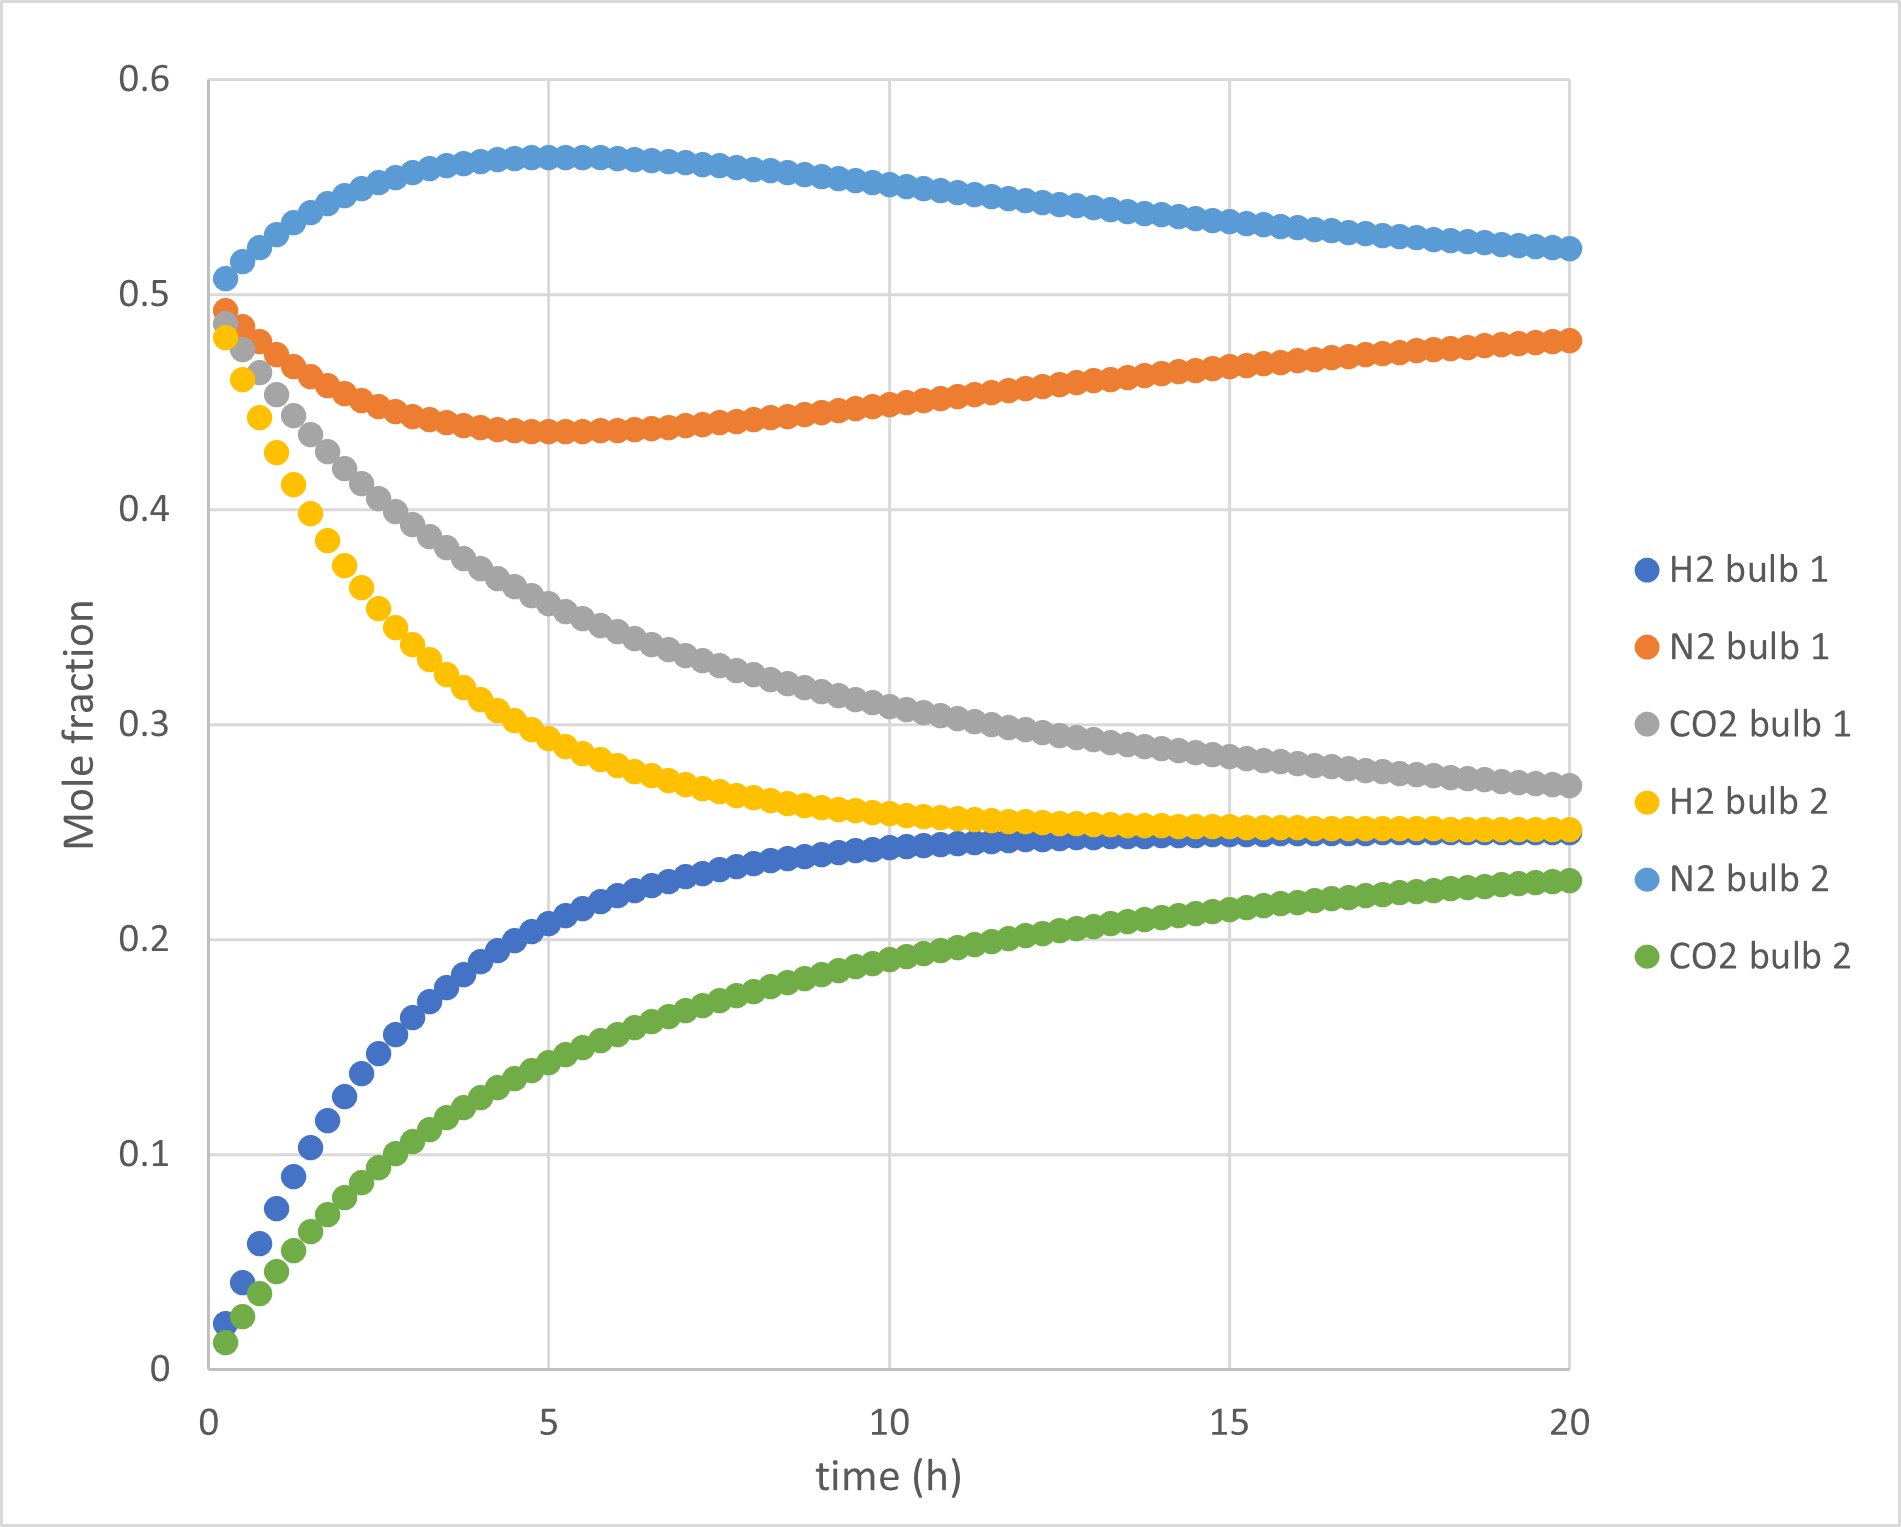
\includegraphics[width=\linewidth]{graph_of_results.png}
\caption{The mole fraction as a function of time (h).}
\label{fig:fig_1}
\end{figure}

\end{document}